\documentclass{article}

\usepackage{booktabs}
\usepackage{tabularx}
\usepackage{hyperref}
\usepackage[a4paper, margin=0.75in]{geometry}
\usepackage{graphicx}
\usepackage{subcaption}
\usepackage{float}

\hypersetup{
    colorlinks=true,       % false: boxed links; true: colored links
    linkcolor=red,          % color of internal links (change box color with linkbordercolor)
    citecolor=green,        % color of links to bibliography
    filecolor=magenta,      % color of file links
    urlcolor=cyan           % color of external links
}

\title{Hazard Analysis\\\progname}

\author{\authname}

\date{}

%% Comments

\usepackage{color}

\newif\ifcomments\commentstrue %displays comments
%\newif\ifcomments\commentsfalse %so that comments do not display

\ifcomments
\newcommand{\authornote}[3]{\textcolor{#1}{[#3 ---#2]}}
\newcommand{\todo}[1]{\textcolor{red}{[TODO: #1]}}
\else
\newcommand{\authornote}[3]{}
\newcommand{\todo}[1]{}
\fi

\newcommand{\wss}[1]{\authornote{magenta}{SS}{#1}} 
\newcommand{\plt}[1]{\authornote{cyan}{TPLT}{#1}} %For explanation of the template
\newcommand{\an}[1]{\authornote{cyan}{Author}{#1}}

%% Common Parts

\newcommand{\progname}{ProgName} % PUT YOUR PROGRAM NAME HERE
\newcommand{\authname}{Team \#, Team Name
\\ Student 1 name
\\ Student 2 name
\\ Student 3 name
\\ Student 4 name} % AUTHOR NAMES                  

\usepackage{hyperref}
    \hypersetup{colorlinks=true, linkcolor=blue, citecolor=blue, filecolor=blue,
                urlcolor=blue, unicode=false}
    \urlstyle{same}
                                


\begin{document}

\maketitle
\thispagestyle{empty}

~\newpage

\pagenumbering{roman}

\begin{table}[hp]
\caption{Revision History} \label{TblRevisionHistory}
\begin{tabularx}{\textwidth}{llX}
\toprule
\textbf{Date} & \textbf{Developer(s)} & \textbf{Change}\\
\midrule
2025-10-02 & Abyan & Scope and Purpose\\
2025-10-02 & Farhan & Critical assumptions made for the project\\
2025-10-01 & Prerna & Add initial version of introduction\\
Date2 & Name(s) & Description of changes\\
... & ... & ...\\
\bottomrule
\end{tabularx}
\end{table}

~\newpage

\tableofcontents

~\newpage

\pagenumbering{arabic}


\section{Introduction}

This document outlines the hazard analysis of the \textbf{Large Event Management System (LEMS)} for the McMaster
Engineering Society (MES). The LEMS is a centralized platform designed to streamline event workflows such as
 \textbf{ticket sales, registrations, waivers, payments, bus/table sign-ups, notifications, and event check-ins}.'
\newline

\noindent
For this deliverable, the analysis will specifically focus on the features within the scope of \textbf{Project B} which include:

\begin{itemize}
    \item Payment System
    \item Role-Centric/Feature-Based Access Control (RBAC/FBAC)
    \item Bus Sign-Ups
    \item RSVP Sign-Ups
    \item Table Sign-Ups
\end{itemize}

\noindent
Hazards in this system refer to conditions or failures that may lead to financial loss, security/privacy breaches,
accessibility failures, or reputational damage for MES and McMaster University. While the system does not directly
involve hardware or pose risks of physical harm, software risks are significant. These include data loss, payment
errors, registration corruption, check-in failures, and unauthorized access to sensitive information.
\newline

\noindent
The purpose of this hazard analysis is to:

\begin{itemize}
    \item Identify risks associated with the Payment, Access Control, and Signup modules.
    \item Define their potential impacts on users, organizers, and the MES organization.
    \item Introduce mitigation strategies by specifying safety and security requirements that
     will guide system design and implementation.
\end{itemize}

\noindent
By proactively addressing these hazards, this analysis ensures the system will be reliable, secure, accessible, and trustworthy for both organizers and attendees.

\section{Scope and Purpose of Hazard Analysis}


The purpose of this hazard analysis is to identify and evaluate potential hazards that could arise during 
the development and operation of the Large Event Management System (LEMS). Since LEMS is a 
software-based platform that supports event registration, ticketing, payments, and participant 
management, hazards are primarily related to data integrity, system availability, security, and user 
interactions. By analyzing these risks early, the project team can define mitigation strategies, 
incorporate safety and security requirements into the design, and reduce the likelihood of 
organizational or reputational harm.

\par
\vspace{1em}

The scope of this analysis covers all major components of LEMS, including the backend services, 
web and mobile applications, and the database. It considers hazards introduced by user error, software 
defects, integration failures across modules, and security vulnerabilities. Hazards that fall outside the 
team’s control, such as third-party cloud hosting failures or issues with external payment providers 
(e.g., Stripe), are acknowledged but not analyzed in detail.

\par
\vspace{1em}

The goals of this hazard analysis are:
\begin{itemize}
  \item To proactively identify risks related to security, data integrity, privacy, and availability in LEMS.
  \item To evaluate the potential consequences of failures, such as data loss, financial errors, or 
        unauthorized access to sensitive information.
  \item To define mitigations or controls that reduce these risks to acceptable levels.
  \item To guide architectural and design decisions and support the definition of non-functional 
        requirements such as reliability, security, and maintainability.
\end{itemize}

This hazard analysis will be refined as the project design evolves, ensuring that new risks are 
addressed as they emerge. It is part of the broader quality assurance process and ensures that LEMS 
meets the standards of safety, security, and reliability expected by the McMaster Engineering Society.

\section{System Boundaries and Components}

The MacSync platform system that the hazard analysis will be conducted on consists of:
\begin{enumerate}
    \item The application that is both web and mobile based, which includes the front-end and back-end made up of the following major components:
    \begin{itemize}
        \item Dashboards (User and Admin)
        \item Payment System
        \item Authentication (Role/Feature Based Access Control)
        \item RSVP Sign-Ups
        \item Bus Sign-Ups
        \item Table Sign-Ups
    \end{itemize}
    \item The PostgreSQL database where all user, admin, event and transaction data will be stored.
    \item The payment module that interfaces with external payment gateways to process ticket payments and refunds.
    \item The notification service that sends automated emails and notifications to users for event details and payment receipts.
\end{enumerate}

The system boundary in the case of the MacSync platform includes components necessary to support event operations for the MES, which includes the entire application, both web and mobile based, along with their subcomponents, the database, payment gateway and notification service. The payment and notification services are controlled by external providers. The payment is controlled by Stripe and the notification service is controlled by Microsoft. However, they remain critical to the function of the system and the overall operation of the platform and thus fall within the system boundary.

\section{Critical Assumptions}

The following assumptions have been identified as critical to the safe and reliable operation of the MacSync platform.

\begin{itemize}
    \item \textbf{Reliable Internet Access:} It is assumed that both attendees and organizers will have access to stable internet connections during registration, payment, and check-in. While temporary connectivity loss may occur, the system must handle these cases gracefully.
    
    \item \textbf{Third-Party Service Availability:} The platform depends on external services such as payment processors (e.g., Stripe, PayPal) and hosting infrastructure. It is assumed these services provide high availability, but the system will still account for outages or delays to prevent complete operational failure.
    
    \item \textbf{Device Compatibility:} It is assumed that attendees will primarily use modern smartphones and organizers will have access to laptops or mobile devices capable of running the dashboard. Reliance on outdated devices or unsupported browsers must be minimized through compatibility testing.
    
    \item \textbf{User Data Accuracy:} The system assumes that users provide correct information (e.g., dietary restrictions, accessibility needs, payment details). However, hazards tied to incorrect or incomplete inputs will be addressed by validation checks.
    
    \item \textbf{Organizational Oversight:} It is assumed that event organizers will actively monitor the system for anomalies (e.g., payment disputes, capacity errors, failed notifications). This system will assist and automate many of the tasks and centralize information, but human oversight is still necessary to manage unexpected situations.
    
    \item \textbf{Security Measures:} It is assumed that standard security practices (encrypted storage, secure authentication, and role-based access control) will be implemented and maintained. Failure to enforce these could expose sensitive student data or enable fraudulent event access.
\end{itemize}


\section{Failure Mode and Effect Analysis}

The Failure Mode \& Effect Analysis (FMEA) is the tool chosen to identify possible hazards within the system. Identifying these hazards will allow the creation of strategies to mitigate them.

\subsection{Hazards Out of Scope}
The following hazards fall outside the control of the dev team however, still have a critical impact on system operations:
\begin{enumerate}
    \item The users mobile device
    \item Hosting provider availability
    \item External payment gateway provider availability
    \item Any External API's hosted by third-party providers (ie. Calendars, Database, OAuth)
\end{enumerate}
These dependecies are all hosted by third party services and therefore the development team cannot control the downtime or availability of them. However, an attempt will be made to mitigate these hazards as much as possible in the case they occur.

\subsection{Failure Modes \& Effects Analysis Table}

\begin{figure}[H]
\begin{subfigure}{\textwidth}
    \centering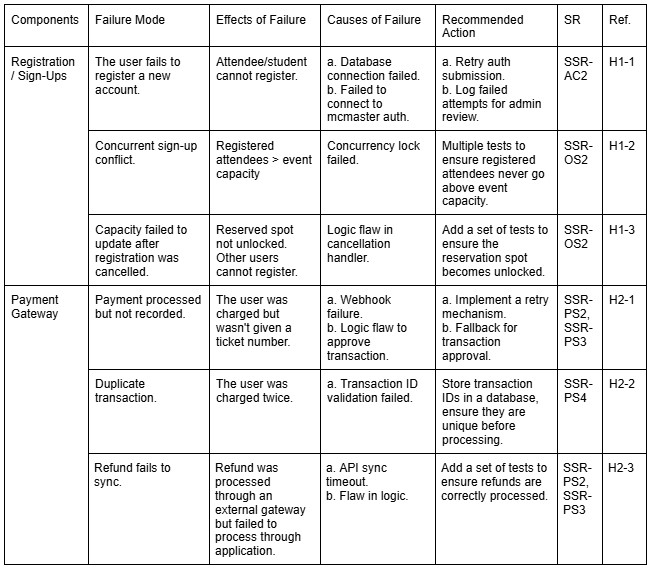
\includegraphics[width=\textwidth]{part1-register_payment.jpg} 
    \caption{FMEA Table Part 1}
\end{subfigure}

\begin{subfigure}{\textwidth}
    \centering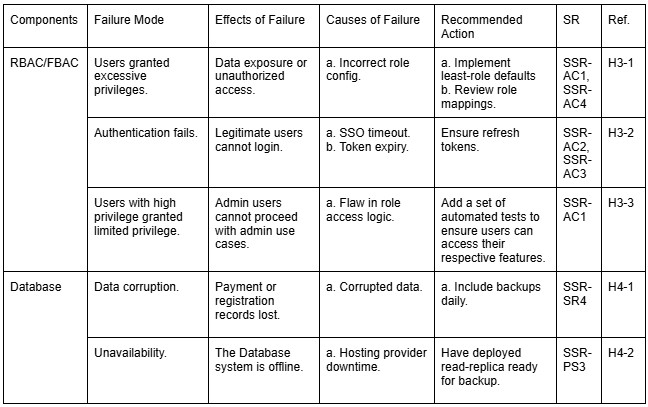
\includegraphics[width=\textwidth]{part2-rbac_db.jpg} 
    \caption{FMEA Table Part 1}
\end{subfigure}

\end{figure}

\section{Safety and Security Requirements}

\wss{Newly discovered requirements.  These should also be added to the SRS.  (A
rationale design process how and why to fake it.)}

\section{Roadmap}

\wss{Which safety requirements will be implemented as part of the capstone timeline?
Which requirements will be implemented in the future?}

\newpage{}

\section*{Appendix --- Reflection}

\wss{Not required for CAS 741}

The purpose of reflection questions is to give you a chance to assess your own
learning and that of your group as a whole, and to find ways to improve in the
future. Reflection is an important part of the learning process.  Reflection is
also an essential component of a successful software development process.  

Reflections are most interesting and useful when they're honest, even if the
stories they tell are imperfect. You will be marked based on your depth of
thought and analysis, and not based on the content of the reflections
themselves. Thus, for full marks we encourage you to answer openly and honestly
and to avoid simply writing ``what you think the evaluator wants to hear.''

Please answer the following questions.  Some questions can be answered on the
team level, but where appropriate, each team member should write their own
response:


\begin{enumerate}
    \item What went well while writing this deliverable? 
    \item What pain points did you experience during this deliverable, and how
    did you resolve them?
    \item Which of your listed risks had your team thought of before this
    deliverable, and which did you think of while doing this deliverable? For
    the latter ones (ones you thought of while doing the Hazard Analysis), how
    did they come about?
    \item Other than the risk of physical harm (some projects may not have any
    appreciable risks of this form), list at least 2 other types of risk in
    software products. Why are they important to consider?
\end{enumerate}

\end{document}